% Reflection in m1 (the x-axis) then in m2 (angle 32 degrees) is the rotation by 64 degrees.
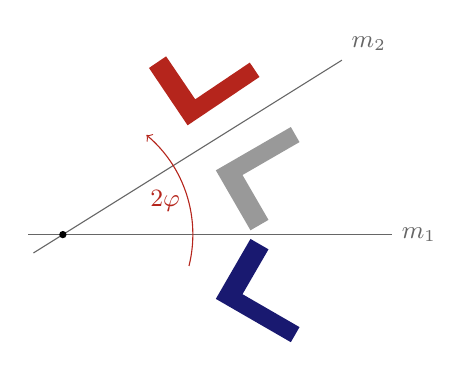
\begin{tikzpicture}[scale=2.2,font=\small]
\draw[black!60] (-0.2,0) -- (1.9,0) node[right] {$m_1$};
\draw[black!60] (-0.170,-0.106) -- (1.611,1.007) node[above right] {$m_2$};
\fill[MidnightBlue] (0.883,-0.371) -- (1.316,-0.621) -- (1.366,-0.534) -- (1.037,-0.344) -- (1.187,-0.085) -- (1.083,-0.025) -- cycle;
\fill[black!40] (0.883,0.371) -- (1.316,0.621) -- (1.366,0.534) -- (1.037,0.344) -- (1.187,0.085) -- (1.083,0.025) -- cycle;
\fill[BrickRed] (0.720,0.631) -- (1.135,0.910) -- (1.079,0.993) -- (0.764,0.781) -- (0.596,1.029) -- (0.497,0.962) -- cycle;
\draw[->,BrickRed] (0.728,-0.181) arc (-14.0:50.0:0.750);
\node[BrickRed] at (0.590,0.192) {$2\varphi$};
\fill (0,0) circle (0.6pt);
\end{tikzpicture}
